\item \subquestionpoints{2} Run \texttt{src/p05\_percept.py} to train
kernelized perceptrons on \texttt{data/ds5\_train.csv}. The code will then test
the perceptron on \texttt{data/ds5\_test.csv} and save the resulting
predictions in the \texttt{src/output} folder. Plots will also be saved in
\texttt{src/output}.  We provide two kernels, a dot product kernel and an
radial basis function (rbf) kernel. One of the provided kernels performs
extremely poorly in classifying the points. Which kernel performs badly and why
does it fail?

\ifnum\solutions=1 {
  \begin{answer}
    \begin{figure}[htbp]
        \begin{subfigure}[b]{0.5\linewidth}
            \centering
            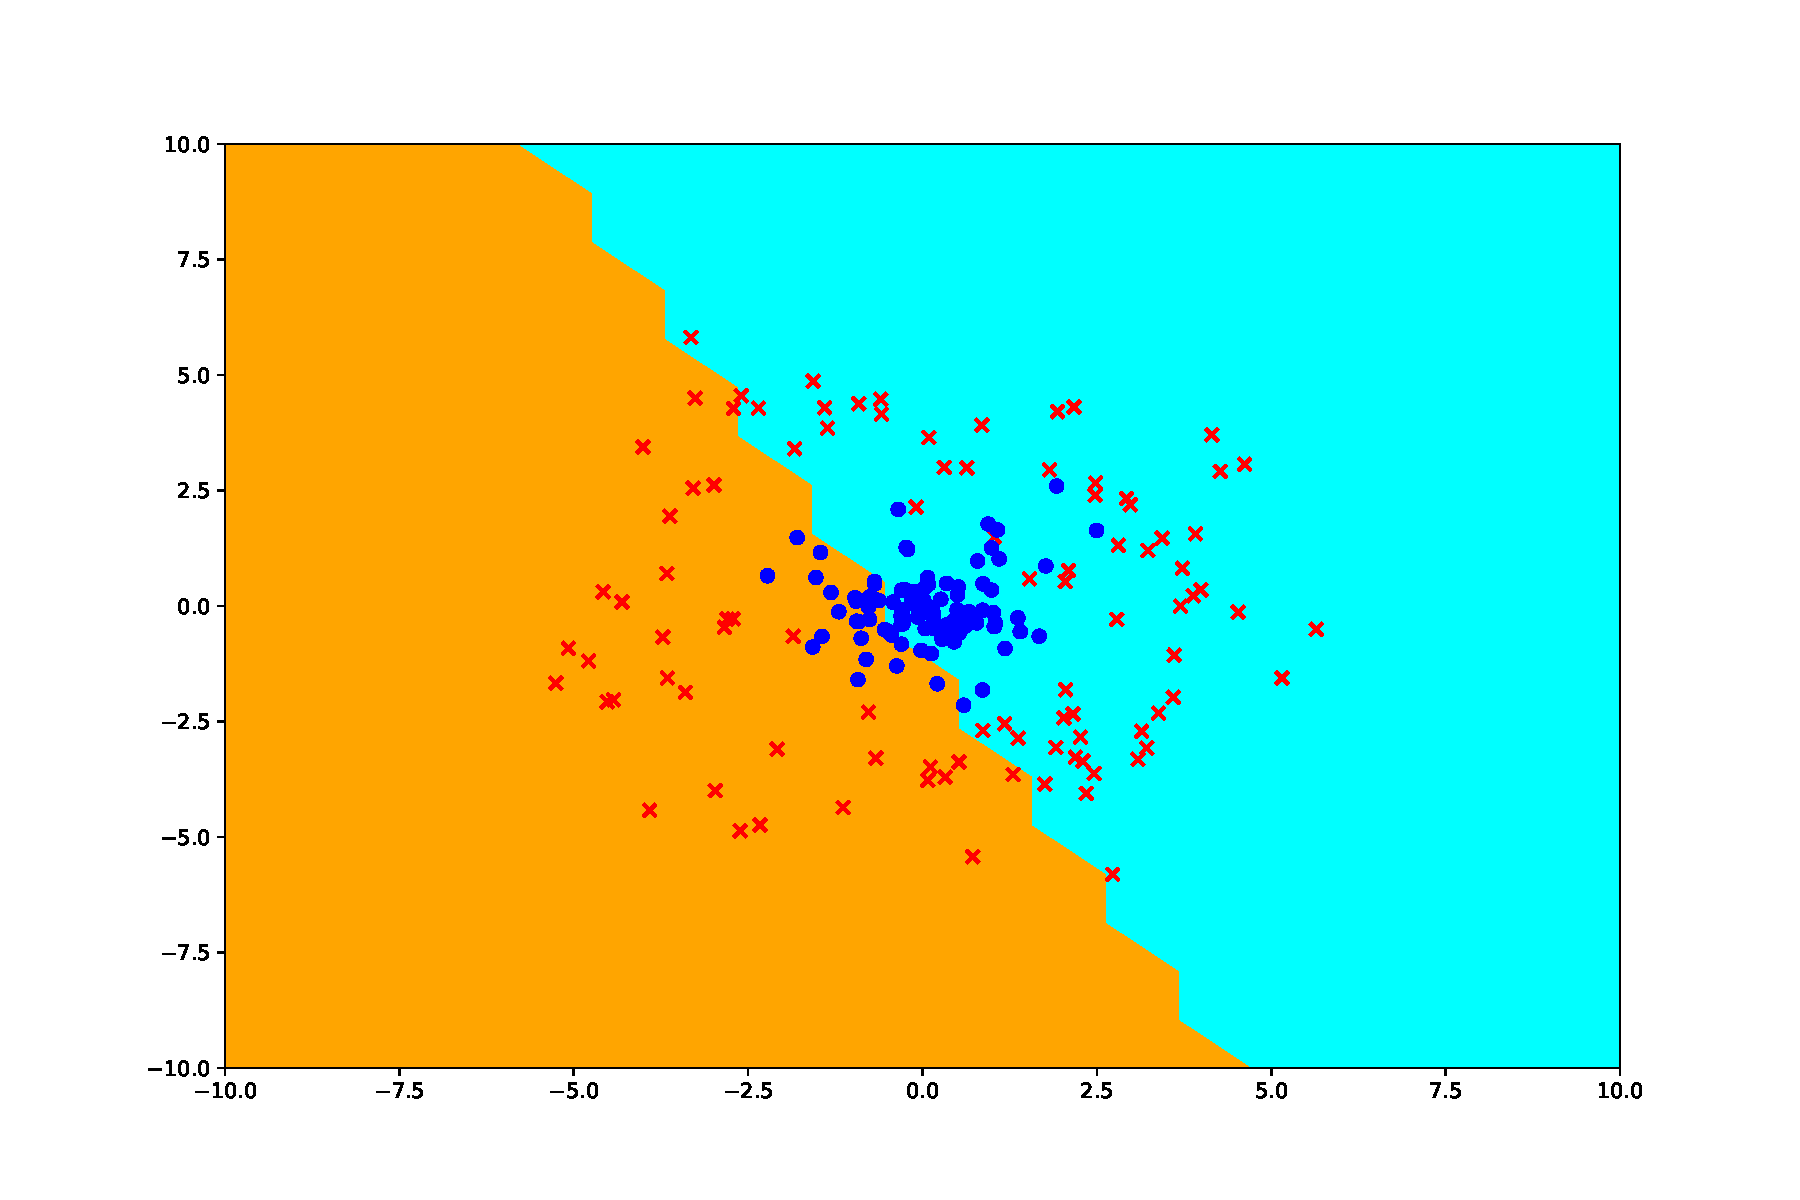
\includegraphics[width=\linewidth]{pics/p05_dot_output.pdf}
            \caption{Dot}
        \end{subfigure}
        \begin{subfigure}[b]{0.5\linewidth}
            \centering
            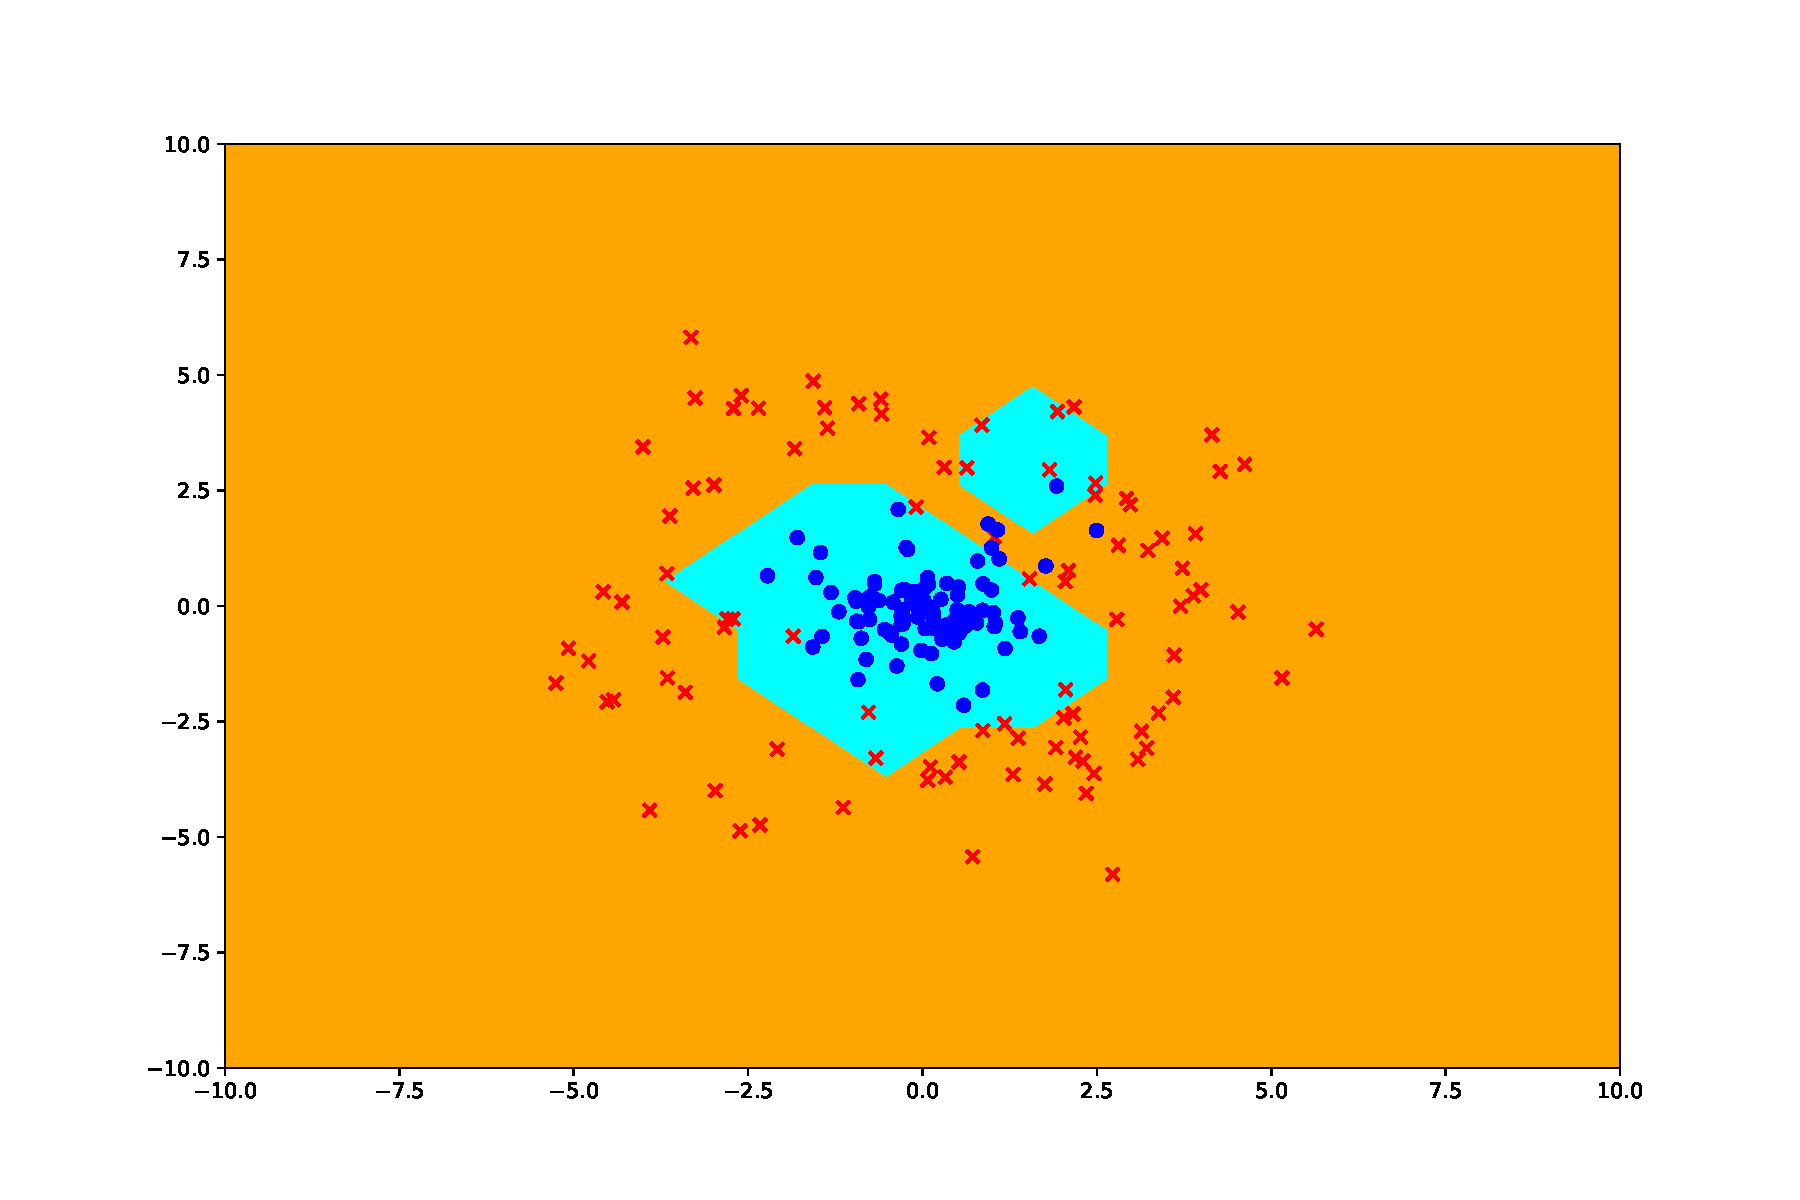
\includegraphics[width=\linewidth]{pics/p05_rbf_output.pdf}
            \caption{RBF}
        \end{subfigure}
    \end{figure}

    The fist performs poorly because using dot product it is equivalent to use $\phi(x^{(i)}) = x^{(i)}$, but the data is not linearly seperable.
\end{answer}

} \fi
